
%%https://tikz.de/polynome/#more-370
\documentclass{standalone}
\usepackage{pgfplots}
\usepgfplotslibrary{colormaps}
\begin{document}
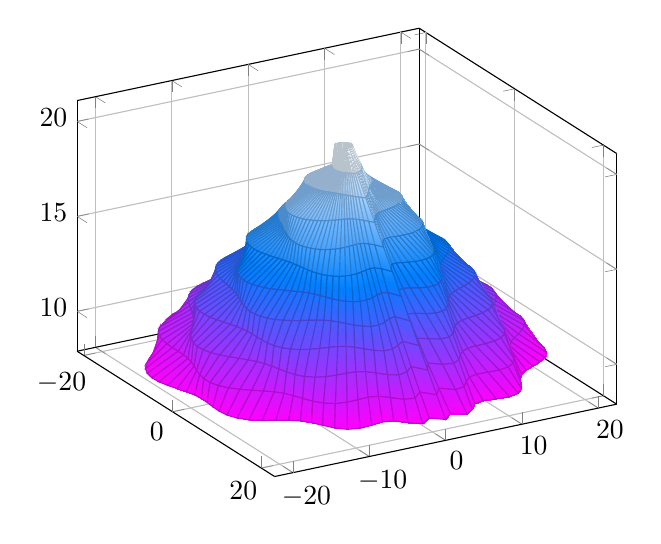
\begin{tikzpicture}
  \begin{axis}[
      data cs = polar,
      grid,
      colormap/cool,
      point meta = -z,
      view = {60}{30} ]
    \addplot3[surf, shader = faceted interp, domain = 0:360,
      samples=100, y domain = 0:11, samples y = 12, z buffer = sort]
        ( {x}, { y*2 + cos(y*2*acos(x/180-1))}, {20-y} );
  \end{axis}
\end{tikzpicture}
\end{document}